\documentclass[11pt]{article}

\usepackage[margin=1in,includefoot]{geometry}
\usepackage{fancyhdr}
\usepackage[colorlinks=true,urlcolor=blue,citecolor=blue]{hyperref}
\usepackage{url}
\usepackage{graphicx}
\usepackage{listings}
\pagestyle{fancy}
\renewcommand\footrulewidth{1pt}
\makeatletter
\g@addto@macro{\UrlBreaks}{\UrlOrds}
\makeatother
\lstset{
   basicstyle=\fontsize{8}{10}\selectfont\ttfamily
}

\begin{document}

\begin{titlepage}

	\begin{center}
	
	\huge ITCS443 Parallel and Distributed Systems\\
	[0.8cm]
	\LARGE Project Report\\
	[0.3cm]
	\Large CUDA - BGR2GRAY and Image Addition\\
	[1.5cm]
	\LARGE Members\\
	[0.5cm]
	\Large Kasidit   	Ruaydee   		   5988117\\
	[0.2cm]
	\Large Pasin        Pubpateeravanich   5988186\\
	[0.2cm] 
	\Large Patthanayu   Rueangdej   	   5988195\\ 
	[0.2cm]
	\Large Nuwat   		Tantbirojn   	   5988240\\    
	[1.5cm]
	\LARGE Presented to\\
	[0.2cm]
	\Large Dr. Putt Sakdhnagool\\
	[1.5cm]
	\Large Faculty of Information and Communication Technology\\
	[0.2cm]
	\Large Mahidol University\\
	[0.2cm]
	\Large 2018
	\begin{figure}[h]
	\centering
	
\includegraphics[scale=0.35]{mu}
	\end{figure}
	
	\end{center}
	
\end{titlepage}

\section{Introduction}\label{sec:intro}
\subsection{Project goal}
To successfully applied CUDA to python in image processing program to see if using CUDA is able to make a program process faster than serial implementation.
\subsection{Why is this project interesting / worth to do?}
We need to prove that if we able to use CUDA to apply parallel processing in any kind of program, the process of a program will be faster than serial implementation program with sequential processing. It's worth doing because if it can guarantees a program to have faster processing, it would be a good thing for us to be able to use it with other codes.


\newpage
\section{Methodology / Algorithm}\label{sec:method}
\subsection*{**Requirement for Pycuda**}
In this project, we implement the source code using Pycharm with Python language. In order to apply CUDA with Python, first we have to install library called Pycuda in the machine which is available on the website below.\\
[0.1cm] 
\url{www.ibm.com/developerworks/community/blogs/jfp/entry/Installing_PyCUDA_On_Anaconda_For_Windows?lang=en&fbclid=IwAR0P1-BGoCtI_tVeT7BbndyprPOG-d08BkCstBf8P_WQOUwkeAMrH1TaGDo}\\
[0.1cm] 
After pycuda is downloaded, continue to install pycuda on the machine through Anaconda prompt/ command prompt by typing the command line “pip install pycuda”\cite{Ibm}.

\begin{figure}[h]
\centering
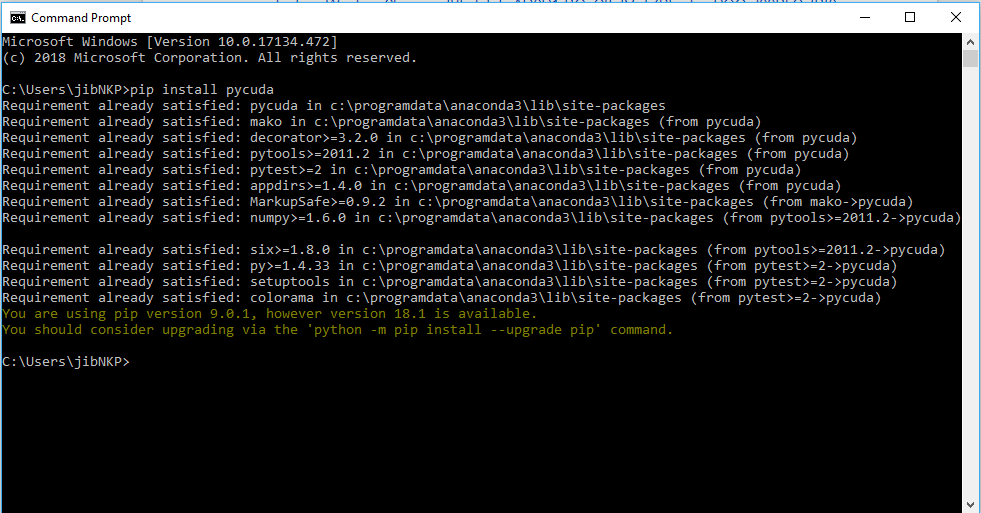
\includegraphics[scale=0.6]{cmd}
\caption{Pycuda Installation}
\end{figure}


\newpage
After the installation is completed, we have to create paths for pycuda to be able to compile on Pycharm.
\begin{lstlisting}
Path1:C:\Program Files\NVIDIA GPU Computing Toolkit\CUDA\v10.0\bin
Path2:C:\Program Files (x86)\Microsoft Visual Studio 14.0\VC\bin
\end{lstlisting}
\begin{figure}[h]
\centering
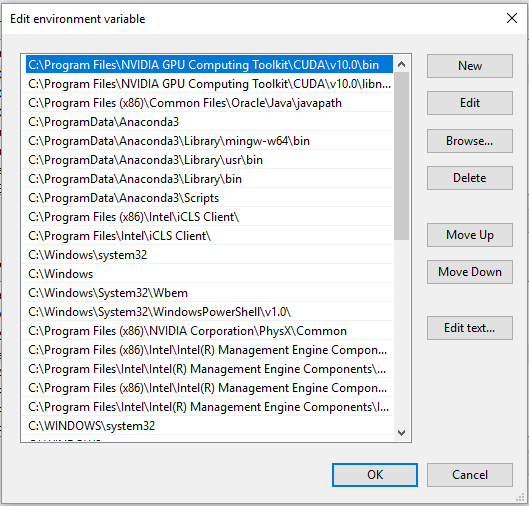
\includegraphics[scale=0.585]{path1}
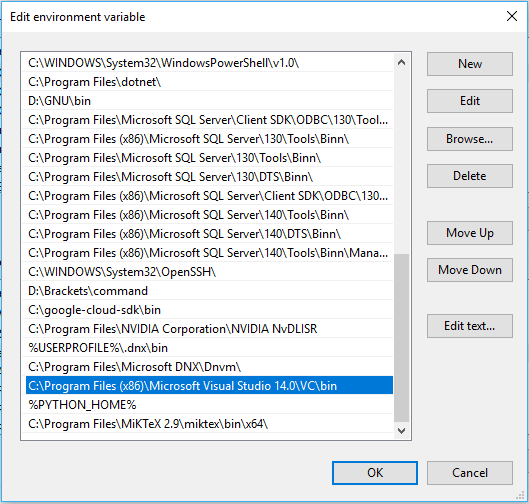
\includegraphics[scale=0.585]{path2}
\caption{Creating paths on the machine}
\end{figure}

\subsection{High-level description of the project / algorithm}
\subsubsection*{BGR2GRAY}
The first program is the image conversion from BGR to Grayscale for 512*512 px image. We create a program that allow user to convert the image from normal image with color to grayscale image. The result of a program will provide the original image and grayscale image.
\subsubsection*{Image addition}
The second program is the image addition for 512*512 px image. We create a program that allow user to create a new image by combining two images together. For the obvious result, user might have to find one image that have transparent background to see the combination between two images.The result of a program will provide 2 of the original images and image that come from the combination of two images.


\newpage
\subsection{Detailed explanation of algorithm}
In both program, we implemented the code that allow us to know the execution time for each code for the comparison and experimental results\cite{KarolisR}. 
\subsubsection{Pycuda\_BGR2GRAY.py}
\subsubsection*{Kernel function}
We created kernel function name’s “bgr2gray”. At the kernel function, we implement a formula to calculate the values of color in each pixel into grayscale. The position of each pixel on the image will be represented by using variable a to represent row and b to represent column\cite{waspinator}\cite{wiki}.

\begin{figure}[h]
\centering
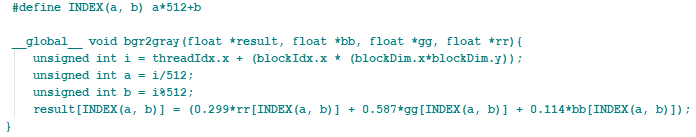
\includegraphics[scale=0.7]{bgr1}
\caption{Kernel function “bgr2gray”}
\end{figure}

\subsubsection*{Main function}
A program will read image and then separate into 3 shades which are blue, green, and red with the same size (262144 comes from 512*512). The variable “result” will copy the array size of one of three shades above and use it to keep the output from kernel. 

\begin{figure}[h]
\centering
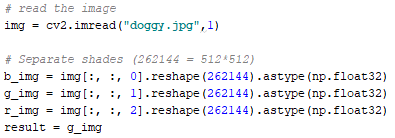
\includegraphics[scale=0.7]{bgr2}
\caption{Read image and separate shades}
\end{figure}


After that, program will call kernel function name’s “bgr2gray” to convert the image into grayscale by passing pointer of b\_img, g\_img, r\_img, and result. After kernel function is finished, program will display two output which are the original image and grayscale image\cite{Ashwin}.

\begin{figure}[h]
\centering
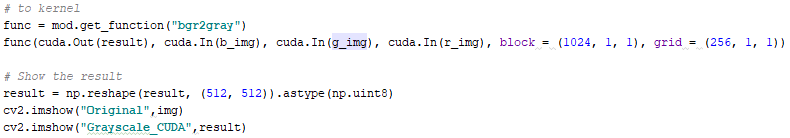
\includegraphics[scale=0.7]{bgr3}
\caption{Call kernel function “bgr2gray” and display output}
\end{figure}


\newpage
\subsubsection{Pycuda\_image\_addition.py}
\subsubsection*{Kernel function}
We created kernel function name’s “addNum”. At the kernel function, we implement a formula to calculate summation of values in each pixel on the first and second image to combine them together. The position of each pixel on the image will be represented by using variable a to represent row and b to represent column.

\begin{figure}[h]
\centering
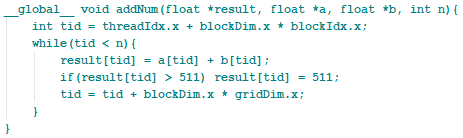
\includegraphics[scale=0.7]{add1}
\caption{Kernel function “addNum”}
\end{figure}

\subsubsection*{Main function}
A program will read two images as grayscale. After that, program will create variables “newimg1” and “newimg2” to receive size of the image which are the same, and variable “n” will be referred to width of the image. The variable “result” will copy the array size of one of newimg above and use it to keep the output from kernel.

\begin{figure}[h]
\centering
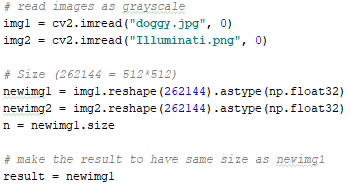
\includegraphics[scale=0.7]{add2}
\caption{Read images and define size}
\end{figure}


After that, program will call kernel function name’s “addNum” to calculate for the summation values of two image and combine them together. After kernel function is finished, program will display three output which are two of the original images and combined image\cite{opencv}.

\begin{figure}[h]
\centering
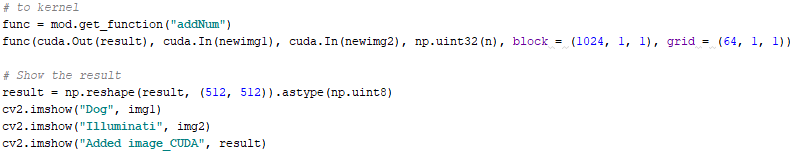
\includegraphics[scale=0.7]{add3}
\caption{Call kernel function “addNum” and display output}
\end{figure}


\newpage
\section{Experiment and results}\label{sec:exp}
\subsection*{CUDA}
We’ve created BGR2GRAY and Image addition with normal python language in order to compare with Pycuda source code and get the experimental result.

\begin{figure}[h]
\centering
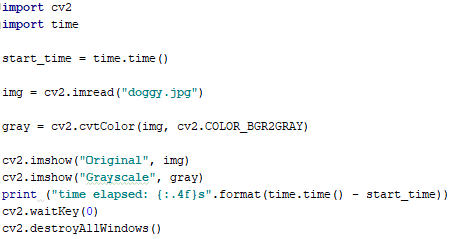
\includegraphics[scale=1]{bgr}
\caption{Python version of BGR2GRAY}
\end{figure}

\begin{figure}[h]
\centering
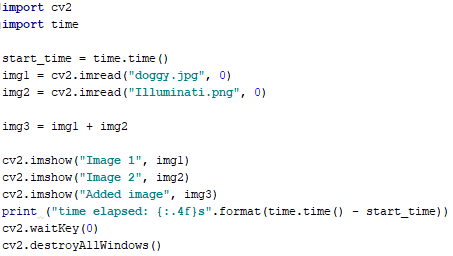
\includegraphics[scale=1]{add}
\caption{Python version of Image addition}
\end{figure}


\newpage
For the image processing result, both programs have the same output which mean that programs that has CUDA applied in it provide the accurate and correct output.

\subsubsection*{Result for BGR2GRAY}
\begin{figure}[h]
\centering
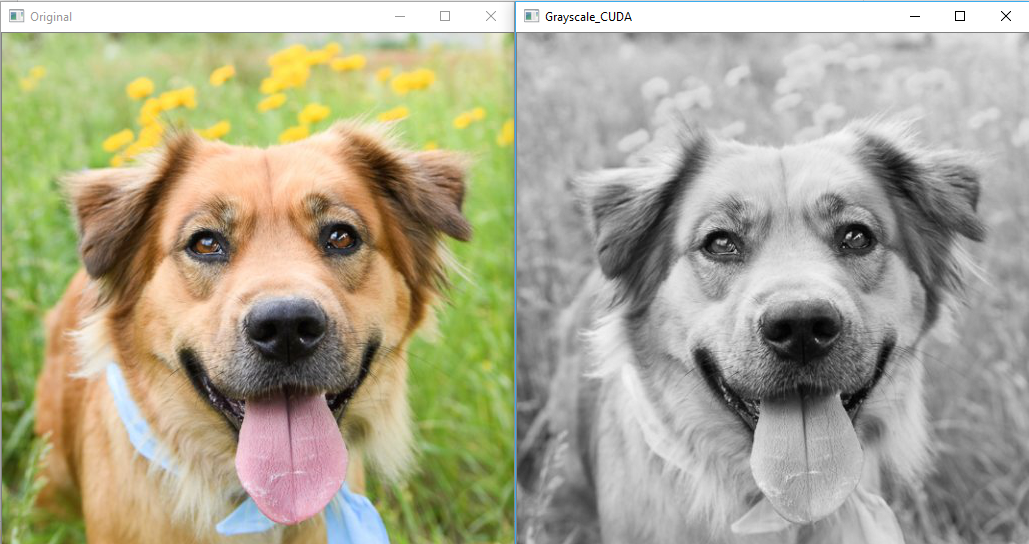
\includegraphics[scale=0.49]{out1}
\caption{Output of Pycuda\_BGR2GRAY}
\end{figure}

\begin{figure}[h]
\centering
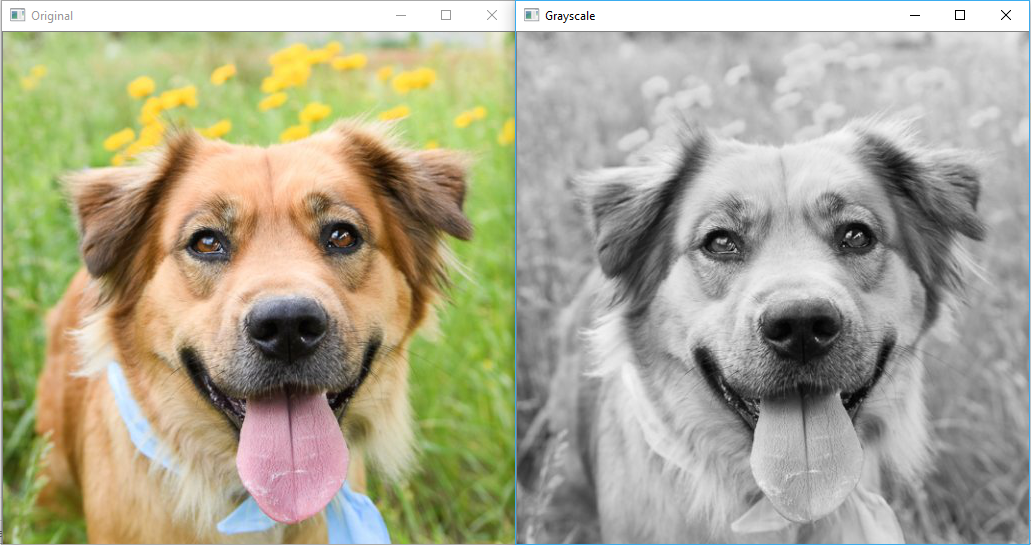
\includegraphics[scale=0.49]{out2}
\caption{Output of BGR2GRAY}
\end{figure}


\newpage
\subsubsection*{Result for Image addition}
\begin{figure}[h]
\centering
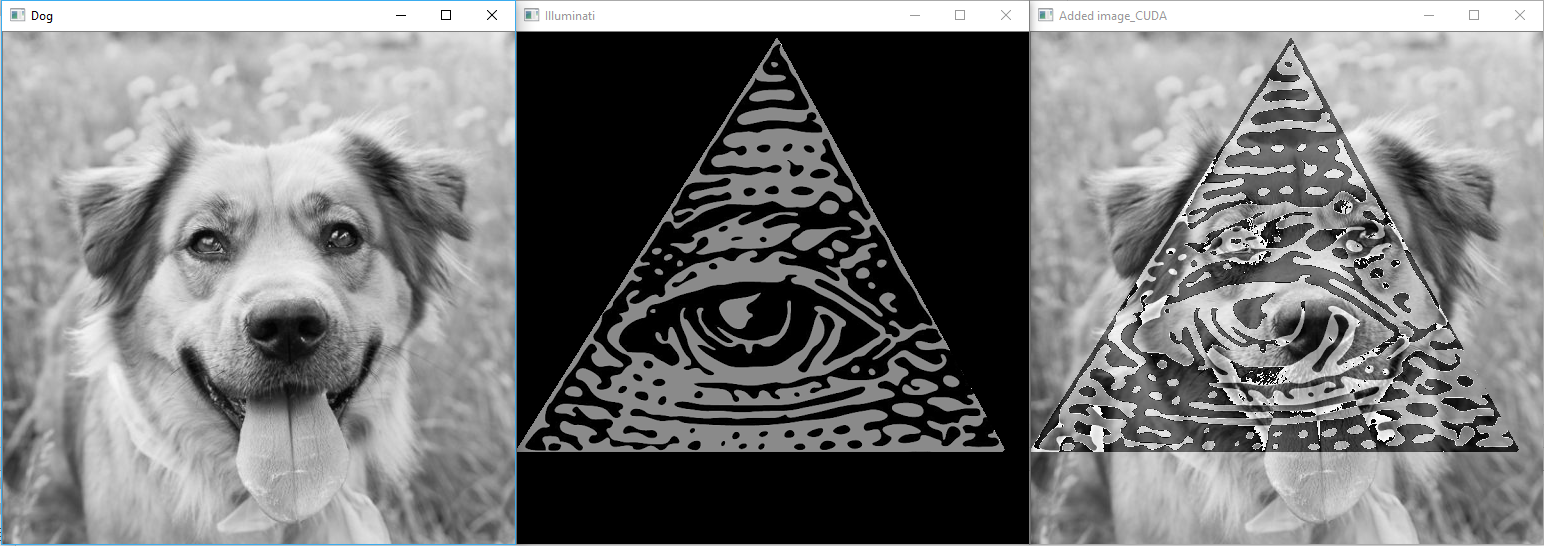
\includegraphics[scale=0.42]{out3}
\caption{Output of Pycuda\_image\_addition}
\end{figure}

\begin{figure}[h]
\centering
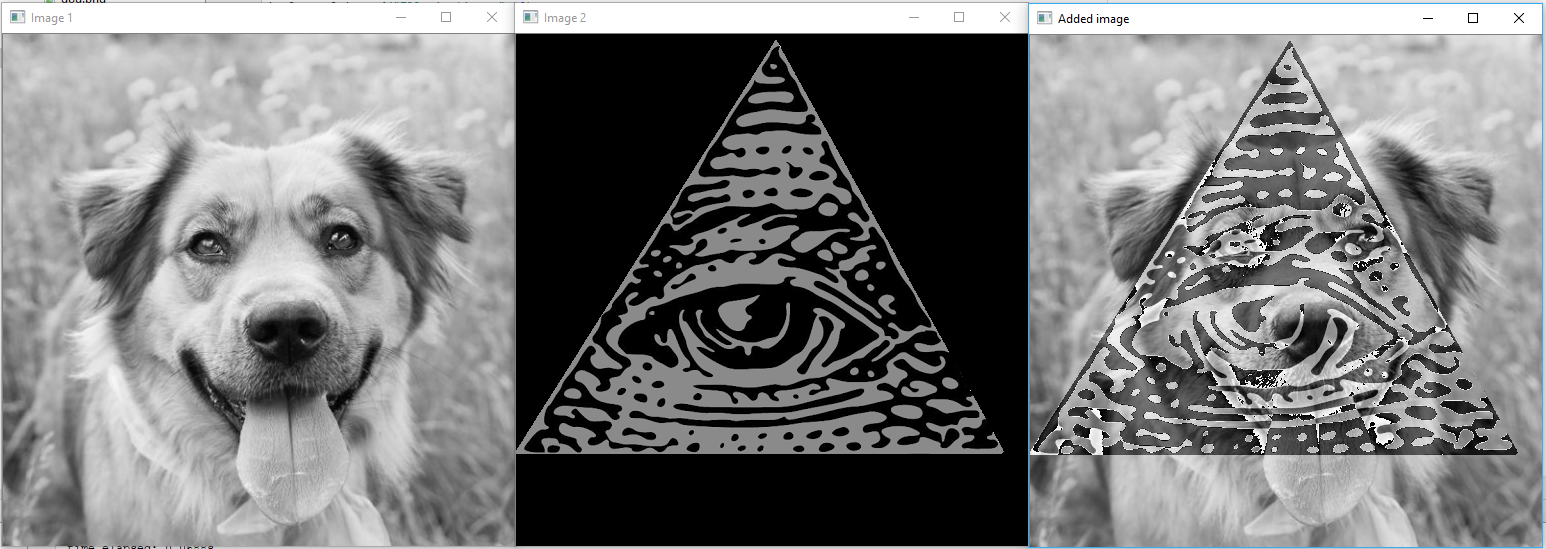
\includegraphics[scale=0.42]{out4}
\caption{Output of Image addition}
\end{figure}


\newpage
On the other hand, the average execution time of Pycuda version and python version almost have the same result. Sometimes Pycuda is faster than Python, and sometimes Python is faster than Pycuda, with little number of different.

\subsubsection*{Execution time for BGR2GRAY}
\begin{figure}[h]
\centering
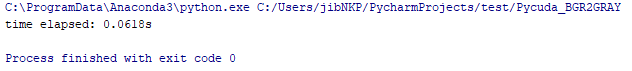
\includegraphics[scale=0.9]{out5}
\caption{Execution time of Pycuda\_BGR2GRAY}
\end{figure}

\begin{figure}[h]
\centering
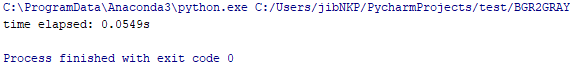
\includegraphics[scale=0.9]{out6}
\caption{Execution time of BGR2GRAY}
\end{figure}

\subsubsection*{Execution time for Image addition}
\begin{figure}[h]
\centering
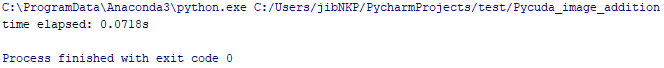
\includegraphics[scale=0.9]{out7}
\caption{Execution time of Pycuda\_image\_addition}
\textsc{}\\[0.5cm]
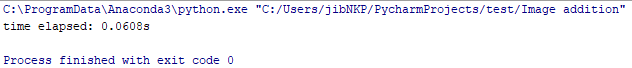
\includegraphics[scale=0.9]{out8}
\caption{Execution time of Image addition}
\end{figure}


\newpage
\section{Discussion and conclusion}\label{sec:dis}
\subsection{Discuss the results of your work}
After the discussion about the result, first we have the same hypothesis of the result for CUDA that it able to make a process faster than normal python program, but the output told us a different story. Due to the curiosity, we‘ve done research more about Pycuda and found that python program that use numpy in the code is already speed up the code. Pycuda is good for accelerate expensive operations. The execution time might not have much different, it usually depend on the size of the images and program flow. There is latency involved in passing the data back and forth across the PCI bus that is only made up for with large data sizes. In conclusion, we can applied cuda to use with python to implement code with accurate output and program execution time between both pycuda and python might not have much different\cite{python}.
\subsection{How to further improve the work}
If we have more time and opportunity to improve the source code for the better result, we would use the advantages of shared memory to apply in the project. Using shared memory could improve a program to be able to work on several images at the same time in multiple thread blocks which might reduce the execution time of a program.


\newpage
\begin{thebibliography}{9}

\bibitem{Ibm} 
Jean Francois Puget. (2016). \textit{Installing PyCUDA On Anaconda For Windows (IT Best Kept Secret Is Optimization).} [online] Available at:
\\\url{https://www.ibm.com/developerworks/community/blogs/jfp/entry/Installing_PyCUDA_On_Anaconda_For_Windows?lang=en&fbclid=IwAR0P1-BGoCtI_tVeT7BbndyprPOG-d08BkCstBf8P_WQOUwkeAMrH1TaGDo}

\bibitem{KarolisR} 
KarolisR. (2016). \textit{How do I time script execution time in PyCharm without adding code every time?.} [online] Stack Overflow. Available at:
\\\url{https://stackoverflow.com/questions/35656239/how-do-i-time-script-execution-time-in-pycharm-without-adding-code-every-time}

\bibitem{waspinator} 
waspinator.  (2012). \textit{How can I convert an RGB image into grayscale in Python?.}  [online] Stack Overflow. Available at: 
\\\url{https://stackoverflow.com/questions/12201577/how-can-i-convert-an-rgb-image-into-grayscale-in-python}

\bibitem{wiki} 
En.wikipedia.org. (2018). \textit{Grayscale.} [online] Available at:
\\\url{https://en.wikipedia.org/wiki/Grayscale#Converting_color_to_grayscale}

\bibitem{Ashwin} 
Ashwin Ashok. (2014). \textit{PyCuda/Examples/SimpleRGB2Gray - Andreas Klöckner's wiki.} [online] Available at:
\\\url{https://wiki.tiker.net/PyCuda/Examples/SimpleRGB2Gray}

\bibitem{opencv} 
Alexander Mordvintsev \& Abid K. (2013). \textit{Arithmetic Operations on Images — OpenCV-Python Tutorials 1 documentation.} [online] Available at:
\\\url{https://opencv-python-tutroals.readthedocs.io/en/latest/py_tutorials/py_core/py_image_arithmetics/py_image_arithmetics.html}

\bibitem{python} 
ardiyu07. (2011). \textit{processing an image using CUDA implementation, python (pycuda) or C++?.} [online] Stack Overflow. Available at:
\\\url{https://stackoverflow.com/questions/4970580/processing-an-image-using-cuda-implementation-python-pycuda-or-c?fbclid=IwAR0Z4tug1Hs7E_3iVMNtS0QKQbKzTU7lLDaEeufVjruk8j_zVrQhk1t2Iug}

\end{thebibliography}

\newpage
\section*{Appendix}\label{sec:app}
\subsection*{Pycuda\_BGR2GRAY.py}
\begin{lstlisting}
# Image convertion to grayscale using Pycuda

import pycuda.driver as cuda
import pycuda.autoinit
from pycuda.compiler import SourceModule
import numpy as np
import cv2
import time # Import for execution time calculation

mod = SourceModule\
  ("""
     #define INDEX(a, b) a*512+b

     __global__ void bgr2gray(float *result, float *bb, float *gg, float *rr){
        unsigned int i = threadIdx.x + (blockIdx.x * (blockDim.x*blockDim.y));
        unsigned int a = i/512;
        unsigned int b = i%512;
        result[INDEX(a, b)] = (0.299*rr[INDEX(a, b)] + 0.587*gg[INDEX(a, b)] + 0.114*bb[INDEX(a, b)]);
    }
    """)

# Start the timer
start_time = time.time()

# read the image
img = cv2.imread("doggy.jpg",1)

# Separate shades (262144 = 512*512)
b_img = img[:, :, 0].reshape(262144).astype(np.float32)
g_img = img[:, :, 1].reshape(262144).astype(np.float32)
r_img = img[:, :, 2].reshape(262144).astype(np.float32)
result = g_img

# to kernel
func = mod.get_function("bgr2gray")
func(cuda.Out(result),cuda.In(b_img),cuda.In(g_img),cuda.In(r_img),block=(1024,1,1),grid=(256,1,1))

# Show the result
result = np.reshape(result, (512, 512)).astype(np.uint8)
cv2.imshow("Original",img)
cv2.imshow("Grayscale_CUDA",result)

# Print execution time result
print ("time elapsed: {:.4f}s".format(time.time() - start_time))
cv2.waitKey(0)
cv2.destroyAllWindows()
\end{lstlisting}


\newpage
\subsection*{Pycuda\_image\_addition.py}
\begin{lstlisting}
# Image addition using Pycuda

import pycuda.driver as cuda
import pycuda.autoinit
from pycuda.compiler import SourceModule
import numpy as np
import cv2
import time # Import for execution time calculation

mod = SourceModule("""
    __global__ void addNum(float *result, float *a, float *b, int n){
        int tid = threadIdx.x + blockDim.x * blockIdx.x;
        while(tid < n){
            result[tid] = a[tid] + b[tid];
            if(result[tid] > 511) result[tid] = 511;
            tid = tid + blockDim.x * gridDim.x;
        }
    }
    """)

# Start the timer
start_time = time.time()

# read images as grayscale
img1 = cv2.imread("doggy.jpg", 0)
img2 = cv2.imread("Illuminati.png", 0)

# Size (262144 = 512*512)
newimg1 = img1.reshape(262144).astype(np.float32)
newimg2 = img2.reshape(262144).astype(np.float32)
n = newimg1.size

# make the result to have same size as newimg1
result = newimg1

# to kernel
func = mod.get_function("addNum")
func(cuda.Out(result),cuda.In(newimg1),cuda.In(newimg2),np.uint32(n),block=(1024,1,1),grid=(64,1,1))

# Show the result
result = np.reshape(result, (512, 512)).astype(np.uint8)
cv2.imshow("Dog", img1)
cv2.imshow("Illuminati", img2)
cv2.imshow("Added image_CUDA", result)

# Print execution time result
print ("time elapsed: {:.4f}s".format(time.time() - start_time))

cv2.waitKey(0)
cv2.destroyAllWindows()

\end{lstlisting}


\newpage
\subsection*{BGR2GRAY.py}
\begin{lstlisting}
import cv2
import time

start_time = time.time()

img = cv2.imread("doggy.jpg")

gray = cv2.cvtColor(img, cv2.COLOR_BGR2GRAY)

cv2.imshow("Original", img)
cv2.imshow("Grayscale", gray)
print ("time elapsed: {:.4f}s".format(time.time() - start_time))
cv2.waitKey(0)
cv2.destroyAllWindows()
\end{lstlisting}


\newpage
\subsection*{Image addition.py}
\begin{lstlisting}
import cv2
import time

start_time = time.time()
img1 = cv2.imread("doggy.jpg", 0)
img2 = cv2.imread("Illuminati.png", 0)

img3 = img1 + img2

cv2.imshow("Image 1", img1)
cv2.imshow("Image 2", img2)
cv2.imshow("Added image", img3)
print ("time elapsed: {:.4f}s".format(time.time() - start_time))
cv2.waitKey(0)
cv2.destroyAllWindows()
\end{lstlisting}

\end{document}